\documentclass{article}
\usepackage[utf8]{inputenc}
\usepackage[margin=1.5in]{geometry}
\usepackage[english]{babel}

\usepackage{graphicx}
\graphicspath{{figures/}}
% \floatplacement{figure}{htb!} % (h)ere (t)op (b)ottom (p)age

\usepackage{amsmath}
\usepackage{nicefrac}

% --- Tables ---
\usepackage{booktabs}
\usepackage{csvsimple}

% --- Fonts ---
\usepackage{fontspec}
\usepackage[babel=true]{microtype}
\defaultfontfeatures{Ligatures=TeX}
\setmainfont{Source Serif Pro}[
  Path = fonts/source-serif-pro/SourceSerifPro-, Extension = .otf,
  Ligatures=TeX,
  UprightFont= Light,
  ItalicFont = LightIt,
  BoldFont   = Regular,
  BoldItalicFont = It]
\setsansfont{Roboto}[
  Ligatures=TeX,
  Path = fonts/roboto/Roboto-, Extension = .ttf,
  UprightFont = Light,
  ItalicFont = LightItalic,
  BoldFont = Regular]
\setmonofont{Source Code Pro}[
  Path = fonts/source-code-pro/SourceCodePro-, Extension = .otf,
  UprightFont = Light,
  BoldFont = Regular]

% --- Citations ---
\usepackage[style=science,sortcites=true,sorting=nyt,backend=biber]{biblatex}
\addbibresource{ref.bib}

% --- Header --- 

\title{A Careful Consideration of the St. Petersburg Paradox}
\author{Alexander R. Koen}
\date{\today}

\begin{document}
\maketitle

\section{The paradox}

If heads appears for the first time on turn $n$, the player is awarded $\$2^n$.


\begin{align*}
\label{eq:1}
  EMV &= \sum_{n=1}^{\infty} \frac{1}{2^{n}}2^n \\
      &= \sum_{n=1}^{\infty}1 \\
      &= \infty
\end{align*}

The St. Petersburg game's possible winnings are geometrically distributed with $Pr(n)=\frac{1}{2}^{n}$, where $Pr(n)$ is the probability of toss $n$ being the first occurrence of heads and thus winning $\$2^n$.

\section{Continuous}

Following probability density function

$$f(x)=\frac{1}{2}2^{-\frac{1}{2}x}$$

\section{Simulating for world}

\begin{table}[h]
  \centering
  \begin{tabular}{cc}
    \toprule
    \textbf{Winnings ($\$2^n$)} & \textbf{Number of People} \\
    \midrule
    1 & 5022 \\
2 & 2521 \\
3 & 1255 \\
4 & 609 \\
5 & 314 \\
6 & 142 \\
7 & 68 \\
8 & 34 \\
9 & 15 \\
10 & 11 \\
11 & 5 \\
12 & 3 \\
13 & 1 \\
14 & 0 \\
15 & 0 \\
16 & 0 \\
17 & 0 \\
    \bottomrule
  \end{tabular}
  \caption{World}
  \label{tab:world}
\end{table}

\begin{figure}[h]
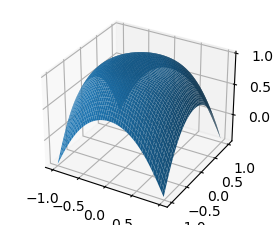
\includegraphics{distribution}
\caption{ Distribution }
\end{figure}

\begin{figure}[h]
  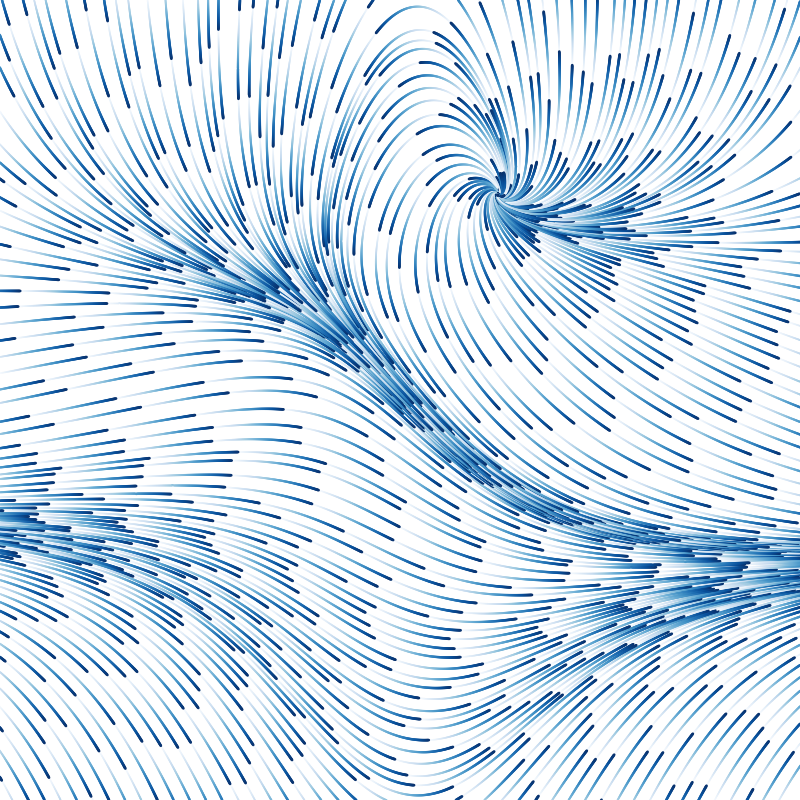
\includegraphics[width=\linewidth]{windmap}
  \caption{ Distribution }
\end{figure}

\section{Lottery}

\begin{table}[h]
  \centering
  \begin{tabular}{cc}
    \toprule
    \textbf{Winnings ($\$2^n$)} & \textbf{Number of People} \\
    \midrule
    $150,000,000$ & $1:292,291,338$\\
    \bottomrule
  \end{tabular}
  \caption{Lottery}
  \label{tab:lotto}
\end{table}

Hello

\printbibliography
\end{document}
